\documentclass[review]{elsarticle} %review=doublespace preprint=single 5p=2 column
%%% Begin My package additions %%%%%%%%%%%%%%%%%%%
\usepackage[hyphens]{url}

  \journal{Tree-Ring Research} % Sets Journal name


\usepackage{lineno} % add
  \linenumbers % turns line numbering on
\providecommand{\tightlist}{%
  \setlength{\itemsep}{0pt}\setlength{\parskip}{0pt}}

\usepackage{graphicx}
\usepackage{booktabs} % book-quality tables
%%%%%%%%%%%%%%%% end my additions to header

\usepackage[T1]{fontenc}
\usepackage{lmodern}
\usepackage{amssymb,amsmath}
\usepackage{ifxetex,ifluatex}
\usepackage{fixltx2e} % provides \textsubscript
% use upquote if available, for straight quotes in verbatim environments
\IfFileExists{upquote.sty}{\usepackage{upquote}}{}
\ifnum 0\ifxetex 1\fi\ifluatex 1\fi=0 % if pdftex
  \usepackage[utf8]{inputenc}
\else % if luatex or xelatex
  \usepackage{fontspec}
  \ifxetex
    \usepackage{xltxtra,xunicode}
  \fi
  \defaultfontfeatures{Mapping=tex-text,Scale=MatchLowercase}
  \newcommand{\euro}{€}
\fi
% use microtype if available
\IfFileExists{microtype.sty}{\usepackage{microtype}}{}
\bibliographystyle{elsarticle-harv}
\usepackage{color}
\usepackage{fancyvrb}
\newcommand{\VerbBar}{|}
\newcommand{\VERB}{\Verb[commandchars=\\\{\}]}
\DefineVerbatimEnvironment{Highlighting}{Verbatim}{commandchars=\\\{\}}
% Add ',fontsize=\small' for more characters per line
\usepackage{framed}
\definecolor{shadecolor}{RGB}{248,248,248}
\newenvironment{Shaded}{\begin{snugshade}}{\end{snugshade}}
\newcommand{\AlertTok}[1]{\textcolor[rgb]{0.94,0.16,0.16}{#1}}
\newcommand{\AnnotationTok}[1]{\textcolor[rgb]{0.56,0.35,0.01}{\textbf{\textit{#1}}}}
\newcommand{\AttributeTok}[1]{\textcolor[rgb]{0.77,0.63,0.00}{#1}}
\newcommand{\BaseNTok}[1]{\textcolor[rgb]{0.00,0.00,0.81}{#1}}
\newcommand{\BuiltInTok}[1]{#1}
\newcommand{\CharTok}[1]{\textcolor[rgb]{0.31,0.60,0.02}{#1}}
\newcommand{\CommentTok}[1]{\textcolor[rgb]{0.56,0.35,0.01}{\textit{#1}}}
\newcommand{\CommentVarTok}[1]{\textcolor[rgb]{0.56,0.35,0.01}{\textbf{\textit{#1}}}}
\newcommand{\ConstantTok}[1]{\textcolor[rgb]{0.00,0.00,0.00}{#1}}
\newcommand{\ControlFlowTok}[1]{\textcolor[rgb]{0.13,0.29,0.53}{\textbf{#1}}}
\newcommand{\DataTypeTok}[1]{\textcolor[rgb]{0.13,0.29,0.53}{#1}}
\newcommand{\DecValTok}[1]{\textcolor[rgb]{0.00,0.00,0.81}{#1}}
\newcommand{\DocumentationTok}[1]{\textcolor[rgb]{0.56,0.35,0.01}{\textbf{\textit{#1}}}}
\newcommand{\ErrorTok}[1]{\textcolor[rgb]{0.64,0.00,0.00}{\textbf{#1}}}
\newcommand{\ExtensionTok}[1]{#1}
\newcommand{\FloatTok}[1]{\textcolor[rgb]{0.00,0.00,0.81}{#1}}
\newcommand{\FunctionTok}[1]{\textcolor[rgb]{0.00,0.00,0.00}{#1}}
\newcommand{\ImportTok}[1]{#1}
\newcommand{\InformationTok}[1]{\textcolor[rgb]{0.56,0.35,0.01}{\textbf{\textit{#1}}}}
\newcommand{\KeywordTok}[1]{\textcolor[rgb]{0.13,0.29,0.53}{\textbf{#1}}}
\newcommand{\NormalTok}[1]{#1}
\newcommand{\OperatorTok}[1]{\textcolor[rgb]{0.81,0.36,0.00}{\textbf{#1}}}
\newcommand{\OtherTok}[1]{\textcolor[rgb]{0.56,0.35,0.01}{#1}}
\newcommand{\PreprocessorTok}[1]{\textcolor[rgb]{0.56,0.35,0.01}{\textit{#1}}}
\newcommand{\RegionMarkerTok}[1]{#1}
\newcommand{\SpecialCharTok}[1]{\textcolor[rgb]{0.00,0.00,0.00}{#1}}
\newcommand{\SpecialStringTok}[1]{\textcolor[rgb]{0.31,0.60,0.02}{#1}}
\newcommand{\StringTok}[1]{\textcolor[rgb]{0.31,0.60,0.02}{#1}}
\newcommand{\VariableTok}[1]{\textcolor[rgb]{0.00,0.00,0.00}{#1}}
\newcommand{\VerbatimStringTok}[1]{\textcolor[rgb]{0.31,0.60,0.02}{#1}}
\newcommand{\WarningTok}[1]{\textcolor[rgb]{0.56,0.35,0.01}{\textbf{\textit{#1}}}}
\usepackage{longtable}
\usepackage{graphicx}
% We will generate all images so they have a width \maxwidth. This means
% that they will get their normal width if they fit onto the page, but
% are scaled down if they would overflow the margins.
\makeatletter
\def\maxwidth{\ifdim\Gin@nat@width>\linewidth\linewidth
\else\Gin@nat@width\fi}
\makeatother
\let\Oldincludegraphics\includegraphics
\renewcommand{\includegraphics}[1]{\Oldincludegraphics[width=\maxwidth]{#1}}
\ifxetex
  \usepackage[setpagesize=false, % page size defined by xetex
              unicode=false, % unicode breaks when used with xetex
              xetex]{hyperref}
\else
  \usepackage[unicode=true]{hyperref}
\fi
\hypersetup{breaklinks=true,
            bookmarks=true,
            pdfauthor={},
            pdftitle={dfoliatR: An R package for detection and analysis of insect defoliation signals in tree rings},
            colorlinks=false,
            urlcolor=blue,
            linkcolor=magenta,
            pdfborder={0 0 0}}
\urlstyle{same}  % don't use monospace font for urls

\setcounter{secnumdepth}{5}
% Pandoc toggle for numbering sections (defaults to be off)


% Pandoc header
\usepackage{booktabs}
\usepackage{longtable}
\usepackage{array}
\usepackage{multirow}
\usepackage{wrapfig}
\usepackage{float}
\usepackage{colortbl}
\usepackage{pdflscape}
\usepackage{tabu}
\usepackage{threeparttable}
\usepackage{threeparttablex}
\usepackage[normalem]{ulem}
\usepackage{makecell}
\usepackage{xcolor}

\usepackage{amsmath}
\usepackage{float}
\usepackage{booktabs}

\begin{document}
\begin{frontmatter}

  \title{\emph{dfoliatR}: An R package for detection and analysis of insect defoliation signals in tree rings}
    \author[a,b]{Christopher H. Guiterman\corref{1}}
   \ead{chguiterman@email.arizona.edu} 
    \author[a,c]{Ann M. Lynch}
   \ead{lyncha@email.arizona.edu} 
    \author[c]{Jodi N. Axelson}
   \ead{jodi.axelson@berkeley.edu} 
      \address[a]{Laboratory of Tree-Ring Research, University of Arizona, 1215 E Lowell St.~Box 210045, Tucson, AZ, 85721}
    \address[b]{Three Pines Forest Research, LLC, PO Box 225, Etna, NH, 03750}
    \address[c]{U.S. Forest Service, Rocky Mountain Research Station, 1215 E Lowell St.~Box 210045, Tucson, AZ, 85721}
    \address[d]{Dept of Environmental Science, Policy \& Management, University of California, Berkeley, Berkeley, CA 94720}
      \cortext[1]{Corresponding Author}
  
  \begin{abstract}
  We present a new R package to provide dendroecologists with tools to infer, quantify, analyze, and visualize growth suppression events in tree rings caused by insect defoliation. The `dfoliatR' library is based on the FORTRAN V program OUTBREAK, and builds on existing resources in the R computing environment. `dfoliatR' expands on OUTBREAK to provide greater control of suppression thresholds, additional output tables, and high-quality graphics. To use `dfoliatR' requires standardized ring-width measurements from insect host trees and an indexed tree-ring chronology from local non-host trees. It performs an indexing procedure to remove the climatic signal represented in the non-host chronology from the host-tree series. It then infers defoliation events in individual trees. Site-level analyses identify outbreak events that synchronously affect a user-defined number or proportion of the host trees. Functions are available for summary statistics and graphics of tree- and site-level series.
  
  \hfill\break
  \end{abstract}
   \begin{keyword} Dendroecology, spruce budworm, Choristoneura, pandora moth, Coloradia pandora Blake, larch-bud-moth
\newpage\end{keyword}
 \end{frontmatter}

\hypertarget{introduction}{%
\section{Introduction}\label{introduction}}

Variation in the width and morphology of annual radial growth rings in trees permits dating and quantification of past forest insect defoliator outbreaks. Defoliation can be distinguished from climate- and other disturbance-related influences by comparing ring-width or other annually-resolved features in the wood of host species to non-host species or to climate records. The effect of defoliation on radial growth of trees has been recognized since the mid-1800s, but it was not until the 1980s that dendrochronology techniques were applied to identify and quantify defoliation events (Lynch, 2012; Speer, 2010; Swetnam et al., 1985). The first studies (Swetnam and Lynch, 1993, 1989; Swetnam et al., 1985) focused on developing historical reconstructions of western spruce budworm (WSBW; \emph{Choristoneura freemani}). The methodology has since been successfully applied to a wide range of defoliator species, most of which are conifer herbivores, and has evolved in sophistication and application to a wide range of ecosystem situations (Lynch, 2012).

The main dendrochronological tool for inferring, dating, and quantifying defoliator outbreaks from tree-ring records has been the software routine OUTBREAK (Holmes and Swetnam, 1986; Swetnam and Lynch, 1989; Swetnam et al., 1985). OUTBREAK computes indices (described later in detail) of suppressed growth by subtracting a detrended and standardized climate series (a ``control'' chronology) from host individual-tree detrended and standardized radial growth series after the host and non-host series have been brought to a common variance. The non-host chronology often consisted of a site chronology developed from non-host tree species, but a gridded climate data point series, like the North American Drought Atlas (Cook and Krusic, 2004) also suffices. If the host and non-host species respond similarly to climate (which can be tested), the derived series retains variability that the host and non-host series do not have in common, generally the insect signal, along with some unexplained variability (noise). The user defines a rule base specifying the magnitude and duration that a period of indexed growth suppression must meet or surpass for a period of suppressed growth to be inferred as a defoliation event at the tree level.

Though powerful, OUTBREAK is outdated and increasingly difficult to use in modern computing environments. It was written in FORTRAN V with inherently severe restrictions, as RAM and disk space were limited at that time (256 kb and 10 MB, respectively) and FORTRAN conventions imposed very strict formatting, file naming, and output conventions. The program provides no graphical interface or capabilities, forcing users to import generated text files into spreadsheet or other software for assessing results and performing analyses. Furthermore, OUTBREAK can only handle one test at a time, creating barriers to batch operation and a large burden for researchers with a datasets including multiple sites. We developed the software library \texttt{dfoliaR} as an \texttt{R}- and \texttt{dplR}-based routine to overcome these issues.

\texttt{dfoliatR} adds to a growing suite of dendrochronology packages the \texttt{R} computing environment (R Core Team, 2019). Stemming from the \texttt{dplR} library (Bunn, 2008) that enables \texttt{R} users to read and write an array of tree-ring data formats, standardize ring width series, build and evaluate chronologies, and perform quality control (to name a few), one can now also measure ring widths from scanned images of prepared samples (Lara et al., 2015; Shi and Xiang, 2019), perform and check crossdating (Bunn, 2010), and perform many analytical tests (Jevšenak and Levanič, 2018; Zang and Biondi, 2015). Tools for assessing stand dynamics and disturbance analyses are under rapid development, with new packages for assessing growth and release events (\texttt{TRADER}: Altman et al., 2014), metrics of growth resilience (\texttt{pointRes}: Maaten-Theunissen et al., 2015), and fire history (\texttt{burnr}: Malevich et al., 2018). The key objective of \texttt{dfoliatR} is to provide tools to identify and analyze insect defoliation and outbreak events by building on the methods employed by OUTBREAK. It capitalizes on the robust software already available in \texttt{R} by using \texttt{dplR} data formats for incoming tree-ring series and providing output data formats embodied by the \texttt{tidyverse} (Wickham et al., 2019) that include efficient data manipulation (Wickham et al., 2020) and graphics (Wickham, 2016).

In this paper, we describe the statistical methods employed by \texttt{dfoliatR}, compare results to those produced by OUTBREAK, and present an example analysis. Users need not have much experience in \texttt{R} to replicate the analyses and graphics as presented. The \texttt{R} code below is executable in an \texttt{R} session once the required libraries are installed and loaded. Support documentation in addition to this paper is provided within the package via standard help menus (accessed by typing \texttt{?} before a function name) and on the package website (\url{https://chguiterman.github.io/dfoliatR/}), which includes up-to-date vignettes that describe various software routines. Code to generate a preprint of this manuscript including the \texttt{R} scripts, and tubular and graphical output is available from \url{https://github.com/chguiterman/dfoliatR_paper}.

\hypertarget{overview-of-the-software}{%
\section{Overview of the software}\label{overview-of-the-software}}

The \texttt{dfoliatR} library requires two sets of tree-ring data to infer defoliation and outbreak events:

\begin{itemize}
\tightlist
\item
  Standardized ring-width series for individual trees of the host species
\item
  Standardized tree-ring chronology from a local non-host species
\end{itemize}

Users can develop these data sets in software of their choosing, such as \texttt{dplR} (Bunn, 2008) or ARSTAN (Cook and Holmes, 1996). It is important that the host-tree data include only one tree-ring series per tree. Both \texttt{dplR} and ARSTAN have options for averaging multiple sample series into a tree-level series.

At the heart of \texttt{dfoliatR} lies two functions: \texttt{defoliate\_trees()} and \texttt{outbreak()}. These identify defoliation events on individual trees (Figure \ref{fig:fig-defol}) and then composite across multiple trees to identify outbreak events (Figure \ref{fig:fig-obr}).

\hypertarget{identifying-defoliation-of-trees}{%
\subsection{Identifying Defoliation of Trees}\label{identifying-defoliation-of-trees}}

The \texttt{defoliate\_trees()} function is the point of entry to the \texttt{dfoliatR} library. It performs two processes, removing climate-related growth signals from the host-tree series and identifying tree-level defoliation events. The climatic or non-defoliation signals in each host-tree series are characterized by a non-host chronology or climate reconstruction. \texttt{dfoiatR} removes that non-defoliation signal by subtracting the non-host series from each host-tree series, which generates a residual index. In OUTBREAK, this residual index was termed the ``corrected'' index. We call it the ``growth suppression index'' (GSI). The GSI is calculated the same as in OUTBREAK for each host tree as
\begin{align}
\textrm{GSI}_{i} = \textrm{H}_{i} - \left( \textrm{NH}_{i} - \overline{\textrm{NH}} \right) \frac{\sigma_{\textrm{H}}}{\sigma_{\textrm{NH}}} \
\end{align}
where H and NH are the host-tree series and the non-host chronology, in year i, respectively. Only the common period between the host-tree series and the non-host chronology are used in Equation 1. The host and non-host chronologies are brought to common variance by scaling the non-host chronology by its mean (\(\overline{\textrm{NH}} \approx 1.0\)) and multiplying by the ratio of host and non-host standard deviations (\(\frac{\sigma_{\textrm{H}}}{\sigma_{\textrm{NH}}}\)), which approximates the variance of the host tree series.

Negative departures in the normalized GSI (NGSI) that surpass user-defined thresholds in duration and magnitude are defined as \emph{defoliation events}. As in OUTBREAK, magnitude is assessed on a single year within the departure sequence. The default setting is -1.28 (in units of standard deviation), which was previously determined to be representative of WSBW effects (Swetnam and Lynch, 1989). Duration is assessed by examining sequences of negative NGSI before and after the year of maximum departure. Each defoliation event is allowed one positive excursion on each side of the maximum departure year. Duration is assessed across the entire sequence that includes up to two positive excursions. The default duration is eight years, as is commonly used in WSBW studies (Swetnam and Lynch, 1989). Different species of defoliation insects vary in the length of defoliation and the degree to which they can suppress tree growth. Researchers can, and should, adjust the duration and magnitude parameters accordingly and critically evaluate the results.

Diverging from OUTBREAK, \texttt{dfoliatR} allows users to extend defoliation events by bridging successive events and also by allowing potentially short-duration events that occur at the end of the series. In cases where two defoliation events are separated by a single year, bridging will link them into a single event (\textbf{Show figure?}). We urge careful use of this option because there is no setting to limit the number or length of potentially bridged events. The series end option can be used in cases when the host trees were actively being defoliated at the time of sampling. This option eliminates the duration parameter for an event at the recent end of the series, but all other thresholds apply. The advantage of this parameter is that it can aid in identifying the start-year for the current defoliation event or outbreak, which is both useful in management and allows the current event to be included in return-interval estimates.

\hypertarget{inferring-outbreak-events}{%
\subsection{Inferring Outbreak Events}\label{inferring-outbreak-events}}

Defoliation of one or a few trees does not constitute an outbreak. To determine when defoliation becomes an \emph{outbreak event}, \texttt{dfoliatR} composites the individual tree defoliation series into a site-level chronology with the \texttt{outbreak()} function. Users have options to define the number and/or the proportion of trees required for an event to be considered an outbreak. Three parameters control whether a defoliation event constitutes an outbreak: the minimum number of trees available, the minimum number of trees recording defoliation, and the percent of trees recording defoliation. The first allows the researcher to make a judgement call as to the confidence ascribed to reduced sample depth toward the ends of their chronologies, thus compensating for the ``fading record problem'' (Swetnam et al., 1999). The second two parameters adjust the scale of defoliation considered to be an outbreak. Absolute numbers of trees and percentages can be applied separately or in conjunction, following filtering conventions in tree ring fire history studies (Malevich et al., 2018). We urge users to carefully consider the choice of absolute numbers in situations where the number of trees represented in the series varies with time, or the choice of percentages when sample size is small.

\hypertarget{evaluation}{%
\section{Evaluation}\label{evaluation}}

\hypertarget{approach}{%
\subsection{Approach}\label{approach}}

We tested \texttt{dfoliatR} against OUTBREAK by comparing NGSI to corrected indices for individual trees and years, defoliation status for individual trees and years, and percentage of trees recording outbreaks at the site level, using standardized ring-width data from eight sites in British Columbia, Colorado, and New Mexico, and author-provided non-host site chronologies.

We detrended host data for both \texttt{dfoliatR} and OUTBREAK using ARSTAN v6.1 (Cook and Holmes, 1996) with default double detrending (128 year wavelength and a 50\% smoothing spline). In both \texttt{dfoliatR} and OUTBREAK we used event thresholds of -1.28 normalized index, 8 years duration, and allowed for events at the end of series in seven of eight sites. These seven sites were sampled during ongoing outbreak events (Swetnam and Lynch, 1993). We found it necessary to be consistent in how we detrended and in what software (e.g., ARSTAN vs \texttt{dplR}) we employed because subtle differences in standardized ring-width indices created between the programs exacerbated differences between \texttt{dfoliatR} and OUTBREAK. In the end, we chose to only use the standardization output files from ARSTAN, which are easily read into \texttt{R} (and then \texttt{dfoliatR}) using the \texttt{dplR} package.

The \texttt{R} code to replicate our comparisons is available from \url{https://github.com/chguiterman/dfoliatR_paper}.

\hypertarget{findings}{%
\subsection{Findings}\label{findings}}

Since both programs employ Equation 1, \texttt{dfoliatR} and OUTBREAK compute identical growth suppression indices at 0.000 precision (Figure \ref{fig:df-obr-1-1}). In all there are 43,280 ring-width indices from 222 trees included in our test. Of these, the programs identified 11,530 years of defoliation. The programs agreed on 92\% of the years, leaving 927 ``difference'' years in which only one program identified defoliation on an individual tree. The differences included 102 events on 85 trees. We carefully inspected each of these events in the full context of each tree's ring series, and categorized the differences as follows

\begin{itemize}
\item
  \emph{Series-end events} (40\% of the total) in which we allowed OUTBREAK to include ``truncated outbreaks'' (for seven sites) at the end of each series. In \texttt{dfoliatR}, this option is controlled by the ``series\_end\_events'' parameter to \texttt{defoliate\_trees()}. In OUTBREAK, the option appears while changing the duration parameter (option 3). When selected, OUTBREAK will include any sequences of negative indices at the either the beginning or the end of each tree series. No thresholds are applied in identifying these as defoliation events. In \texttt{dfoliatR}, the negative sequences are evaluated as with any other possible defoliation, but the duration threshold is omitted. Each of the 13 events included in these differences did not meet the ``max\_reduction'' parameter (-1.28 NGSI) in \texttt{dfoliatR} and were excluded. In two cases, OUTBREAK included events at the beginning of the series where \texttt{dfoliatR} does not allow truncated events. In four cases, OUTBREAK omitted the last year of the series because it was positive. In two cases, \texttt{dfoliatR} omitted possible events because it had already included a positive NGSI excursion after the ``max\_reduction'' year, and since it will only allow one excursion on either side of the max year, the events were omitted due to short duration.
\item
  \emph{Sequential events} (36\%) in which OUTBREAK omitted events that occur one year prior or one year following an identified event. OUTBREAK selects the event with the greatest negative index year. On two trees, OUTBREAK omitted two of three sequential events. \texttt{dfoliatR} allows all such events. While inspecting these differences, we added an option to \texttt{defoiate\_trees()} that would ``bridge'' between sequential events, making them into single, long events. We felt that this was ecologically justified, especially for studies of WSBW, because the insect will occasionally maintain minor defoliation f individuals for decades even while not in an outbreak phase.
\item
  \emph{Undetermined differences} (22\%) occurred in cases where OUTBREAK omitted events without clear cause.
\item
  \emph{Rounding} (2\%) differences in the indices either omitted or cut short events on two trees. In both cases the indices were very close to zero.
\end{itemize}

Our inspections revealed what we believe are short-comings in how OUTBREAK identifies defoliation events on individual trees. In every one of the 102 cases we inspected, we felt that \texttt{dfoliatR} provided a more biologically and statistically appropriate assessment of defoliation.

and use them to infer identical tree-level outbreak events, including onset and termination dates and date and magnitude of the maximum growth suppression when \texttt{dfoliatR} bridging matches the OUTBREAK protocols. Once the issues with ARSTAN (described earlier) were resolved, dfoliatR and OUTBREAK produced identical indices at 0.000 precision.

When inferring outbreak events at the tree level, our initial results did not always match OUTBREAK, leading to development of the bridging option. Identifying a minimum within a period while allowing for positive excursions is a tricky computation. OUTBREAK deliberately disallows back-to-back events -- after a minimum value within a period of negative values, a second positive index terminates an event. OUTBREAK does not allow a period of highly negative values to be appended to an earlier outbreak if the intervening period is 1 year, even if those negative values fall below the minimum in the earlier period. Due in large part to reconstructions using OUTBREAK (see papers cited by Lynch, 2012), we now know considerably more about forest defoliator outbreak regimes than we did in the 1980s when OUTBREAK was written. We think that two prolonged events separated by a single year should in some situations be considered a single outbreak at both the tree and site levels. This is particularly relevant to western spruce budworm and spruce budworm (\emph{C. fumiferana}), for which regimes have been reconstructed for several geographic areas and for which researchers and forest health experts have gained considerable knowledge (\textbf{Sanders et al.~1985, Brookes et al.~1987 and many later publications}). We now know that the greatest growth suppression often occurs late in the outbreak due to cumulative effects (\textbf{rrr}). We developed the bridging option to permit these periods to be linked to preceding events separated by a single year.

Bridging operates at the tree level in \texttt{dfoliatR}, and these effects generally have minor effects on site-level reconstructions (\textbf{Fig.Bridging}). Occasionally site-level events are inferred differently (\textbf{Table.Bridging}), and this can affect return interval and duration statistics.

\hypertarget{best-practice-recommendations}{%
\subsection{Best Practice Recommendations}\label{best-practice-recommendations}}

We encourage authors to report software and library version numbers and download dates where applicable. This is standard practice for statistical packages, but has often been ignored for R- and dplR-based analyses. R-based software evolves over time, and results cannot always be replicated if the software versions are unknown. Similarly, significant changes (especially fixes) imply that re-analysis of data might differ from earlier published results and interpretations. Wherever possible, refereed publications supporting the software should be cited. Our experience with ARSTAN demonstrates the importance of adopting this practice. In the United States, analytic methods not documented thusly and supported by the literature might be questioned if the results are used in a National Environmental Protection Act (NEPA) process.

We recommend that researchers compare dfoliatR results with and without bridging, and see which option agrees best with known insect biology and ecology. Bridging may be a logical choice for insects with prolonged non-outbreak periods, such as western spruce budworm, but not for situations where impacted stands barely recover from one outbreak before another begins, such as occurs with pine processionary caterpillars (\emph{Thaumetopoea pityocampa} (Lepidoptera: Thaumetopoeidae)) (\textbf{Carus 2004, 2009}).

\hypertarget{availability-and-installation}{%
\section{Availability and installation}\label{availability-and-installation}}

The \texttt{dfoliatR} library (Guiterman et al., 2020) is provided free and open source from the Comprehensive R Archive Network (CRAN; \url{https://cran.r-project.org/}). To install \texttt{dfoliatR} from CRAN use

\begin{Shaded}
\begin{Highlighting}[]
\KeywordTok{install.packages}\NormalTok{(}\StringTok{"dfoliatR"}\NormalTok{)}
\end{Highlighting}
\end{Shaded}

In each \texttt{R} session, \texttt{dfoliatR} can be loaded via

\begin{Shaded}
\begin{Highlighting}[]
\KeywordTok{library}\NormalTok{(dfoliatR)}
\end{Highlighting}
\end{Shaded}

Development versions of \texttt{dfoliatR} are available on GitHub and installed using the \texttt{devtools} library,

\begin{Shaded}
\begin{Highlighting}[]
\NormalTok{devtools}\OperatorTok{::}\KeywordTok{install_github}\NormalTok{(}\StringTok{"chguiterman/dfoliatR"}\NormalTok{)}
\end{Highlighting}
\end{Shaded}

Issues, bug reports, and ideas for improving \texttt{dfoliatR} can be posted to \url{https://github.com/chguiterman/dfoliatR/issues}. As an Open Source library, we welcome and encourage community involvement in future development. The best ways to contribute to \texttt{dfoliatR} are through standard GitHub procedures or by contacting the first author.

\hypertarget{example-usage}{%
\section{Example Usage}\label{example-usage}}

In \texttt{dfoliatR} we provide two sets of tree-ring data to aid users in exploring the functions, graphics, and outputs. Each set consists of individual host-tree series, standardized using 50-year splines with a 50\% frequency response, and a local non-host chronology. The non-host ring-width data were standardized using 150-year splines with a 50\% frequency response. The non-host chronologies were averaged following standard procedures (Speer, 2010). Host trees from Demijohn Peak (DMJ; 2902 m asl) in the San Juan Mountains of southern Colorado include Douglas-fir (\emph{Pseudotsuga menziesii}) compared against a local non-host ponderosa pine (\emph{Pinus ponderosa}) chronology (Ryerson et al., 2003). The East Fork site (EF; 2580 m asl) in the Jemez Mountains of northcentral New Mexico include Douglas-fir and white fire (\emph{Abies concolor}) host trees and a ponderosa pine non-host chronology (Swetnam and Lynch, 1993).

\hypertarget{tree-level-defoliation-events}{%
\subsection{Tree-Level Defoliation Events}\label{tree-level-defoliation-events}}

To assess defoliation of trees, we begin with a set of standardized host-tree series and a local non-host chronology or climate reconstruction. First, the \texttt{dfoliatR} library needs to be loaded (after installation as above) and the included datasets can be loaded. The function \texttt{defoliate\_trees()} performs the GSI indexing procedure on each host-tree series and then identifies defoliation events.

\begin{Shaded}
\begin{Highlighting}[]
\CommentTok{## Load the package}
\KeywordTok{library}\NormalTok{(dfoliatR)}

\CommentTok{## Load data}
\KeywordTok{data}\NormalTok{(}\StringTok{"dmj_h"}\NormalTok{) }\CommentTok{# host tree series}
\KeywordTok{data}\NormalTok{(}\StringTok{"dmj_nh"}\NormalTok{) }\CommentTok{# non-host chronology}
\CommentTok{# View data structure for any data object via }
\CommentTok{# "View(dmj_h)" or "head(dmj_h)"}

\CommentTok{## Calculate indices, identify defoliation events}
\NormalTok{dmj_defol <-}\StringTok{ }\KeywordTok{defoliate_trees}\NormalTok{(}\DataTypeTok{host_tree =}\NormalTok{ dmj_h,}
                             \DataTypeTok{nonhost_chron =}\NormalTok{ dmj_nh,}
                             \DataTypeTok{duration_years =} \DecValTok{8}\NormalTok{,  }
                             \DataTypeTok{max_reduction =} \FloatTok{-1.28}\NormalTok{, }
                             \DataTypeTok{bridge_events =} \OtherTok{TRUE}\NormalTok{, }
                             \DataTypeTok{series_end_event =} \OtherTok{TRUE}\NormalTok{, }
                             \DataTypeTok{list_output =} \OtherTok{FALSE}\NormalTok{) }
\end{Highlighting}
\end{Shaded}

The result of running \texttt{defoliate\_trees()} is long-format (stacked) data frame with five variables: ``year'', ``series'', ``gsi'', ``ngsi'', and ``defol\_status.'' The ``gsi'' variable is the ``corrected'' tree-level growth suppression index. It was normalized or scaled into z-scores to produce ``ngsi'', which is used to identify defoliation events. The ``defol\_status'' column provides a set of character strings, ``nd'' for non-defoliation year, ``defol'' for a defoliation year, ``max\_defol'' for the year of maximum suppression (that acts as the basis for individual events), ``bridge\_defol'' to identify years that link subsequent events (only one is present at DMJ), and ``series\_end\_defol'' to identify defoliation at the present-end of the series. Selecting \texttt{list\_output\ =\ TRUE} provides a list-object of data frames, each with the \texttt{rwl} object that combines the host tree and non-host chronology and the columns created in \texttt{defoliate\_trees()}. This option is not used by subsequent functions in \texttt{dfoliatR}, but researchers can examine it to check the results of the GSI calculation (Equation 1).

We can assess the results of running \texttt{defoliate\_trees()} through graphical and table outputs. The function \texttt{get\_defol\_events()} will provide a list of every defoliation event for every tree, with the corresponding mean ``ngsi'' value. A summary table of the results for each tree is produced by \texttt{defol\_stats()} (Table \ref{tab:tbl-defol}).

\begin{Shaded}
\begin{Highlighting}[]
\KeywordTok{defol_stats}\NormalTok{(dmj_defol)}
\KeywordTok{View}\NormalTok{(dmj_defol)}
\end{Highlighting}
\end{Shaded}

The \texttt{plot\_defol()} function produces a ``ggplot'' graphics object with line segments showing the measured sequence of each series and a filled segment for each identified defoliation event (Figure \ref{fig:fig-defol}). The defoliation segments are colored by their relative severity based on their average NGSI value. The default cut-off values between ``Severe'' and ``Moderate'' is the overall mean across all events and between ``Moderate'' and ``Minor'' is the first quartile. Users can define these breaks to suit their needs.

\begin{Shaded}
\begin{Highlighting}[]
\KeywordTok{plot_defol}\NormalTok{(dmj_defol)}
\CommentTok{## This creates a ggplot object, so additions can }
\CommentTok{## be made to adjust plotting themes and}
\CommentTok{## aesthetics, like color.   }
\CommentTok{## For more on the features of ggplot:}
\CommentTok{## https://ggplot2.tidyverse.org/}
\KeywordTok{library}\NormalTok{(ggplot2)}
\KeywordTok{plot_defol}\NormalTok{(dmj_defol) }\OperatorTok{+}
\StringTok{  }\KeywordTok{scale_color_manual}\NormalTok{(}\DataTypeTok{values =} \KeywordTok{c}\NormalTok{(}\StringTok{"red"}\NormalTok{, }\StringTok{"orange"}\NormalTok{, }\StringTok{"purple"}\NormalTok{))}
\end{Highlighting}
\end{Shaded}

These basic output functions aid in assessing the sensitivity of input parameters to \texttt{defoliate\_trees()} including the duration and magnitude thresholds for identifying defoliation events. Using \texttt{plot\_defol()} also provides a direct assessment of the between-tree variability in deflation. For further analyses, we composite the host-tree defoliation series to the site level using \texttt{outbreak()}.

\hypertarget{site-level-events}{%
\subsection{Site-Level Events}\label{site-level-events}}

Once we have identified defoliation events on individual trees, we can infer outbreak events at the site level. The function \texttt{outbreak()} acts to composite tree-level defoliation series into a single chronology, with input parameters that control thresholds in the number and proportions of trees recording a defoliation event.

\begin{Shaded}
\begin{Highlighting}[]
\CommentTok{## Use the defol object "dmj_defol" created above}
\NormalTok{dmj_obr <-}\StringTok{ }\KeywordTok{outbreak}\NormalTok{(dmj_defol,}
                    \DataTypeTok{filter_min_series =} \DecValTok{3}\NormalTok{,}
                    \DataTypeTok{filter_min_defol =} \DecValTok{1}\NormalTok{,}
                    \DataTypeTok{filter_perc =} \DecValTok{25}\NormalTok{)}
\end{Highlighting}
\end{Shaded}

Input parameters to \texttt{outbreak()} include ``filter\_min\_series'' to control the chronology cut-off points with regard to sample depth, ``filter\_min\_defol'' and ``filter\_perc'' to control the minimum number and percent of trees, respectively, recording a defoliation event in a given year. \texttt{Outbreak()} produces a new data frame with eight variables: ``year'', ``num\_defol'', ``percent\_defol'', ``num\_max\_defol'', ``mean\_gsi'', ``mean\_ngsi'', and ``outbreak\_status.'' All of these variables are populated regardless of an inferred outbreak event, providing a continuous disturbance chronology. The ``num\_max\_defol'' variable counts the number of trees recording their maximum defoliation in a given year. The ``mean\_gsi'' and ``mean\_ngsi'' variables provide averages of these indices across all available trees. Finally, the ``outbreak\_status'' column shows whether an outbreak event is inferred (``outbreak'') or not (``not\_obr'').

The default plotting function to visualize results form \texttt{outbreak()} creates a three-panel graph showing the mean site-level chronology, the percent of trees recording a defoliation, and the sample depth over time (Figure \ref{fig:fig-obr}).

\begin{Shaded}
\begin{Highlighting}[]
\KeywordTok{plot_outbreak}\NormalTok{(dmj_obr, }\DataTypeTok{disp_index =} \StringTok{"mean_gsi"}\NormalTok{)}
\end{Highlighting}
\end{Shaded}

Inferred outbreak events are shown in the top panel of Figure \ref{fig:fig-obr} as the filled-in spaces. Users can change the time series in this panel with the ``disp\_index'' parameter, choosing between the mean NGSI (the default) or GSI.

A summary table of the inferred outbreak events is generated by the \texttt{outbreak\_stats()} function (Table \ref{tab:tbl-obr}).

\begin{Shaded}
\begin{Highlighting}[]
\NormalTok{dmj_obr_stats <-}\StringTok{ }\KeywordTok{outbreak_stats}\NormalTok{(dmj_obr)}
\end{Highlighting}
\end{Shaded}

The output table from \texttt{outbreak\_stats()} shows the start and end years of each event, along with their corresponding duration, the number and percent of trees in defoliation at the start of the event, the the number of trees recording the outbreak event (in part or full), the minimums of the mean GSI and NGSI indices, and two points of ``peak defoliation.'' The first, ``peak\_outbreak\_year,'' is the year in which the greatest number of trees is recording the outbreak, and the second, ``peak\_defol\_year,'' is the year in with the lowest average NGSI. These output variables provide a array of options for assessing basic metrics of the insect defoliation regime, including interval analyses:

\begin{Shaded}
\begin{Highlighting}[]
\CommentTok{## calculate mean return interval for outbreak start years}
\NormalTok{intervals <-}\StringTok{ }\KeywordTok{diff}\NormalTok{(dmj_obr_stats}\OperatorTok{$}\NormalTok{start)}
\KeywordTok{mean}\NormalTok{(intervals) }\CommentTok{## 51.2}
\end{Highlighting}
\end{Shaded}

\hypertarget{conclusions}{%
\section{Conclusions}\label{conclusions}}

\begin{itemize}
\tightlist
\item
  Encourage use of \texttt{dfoliatR} over OUTBREAK -- more acruate, greater user control, more easily conduct sensitivity tests to evaluate paramters, data, and ecological patterns
\item
  Facilitates high-levelr statistical analyses by easily transfering to other libraries (MASS, etc.)
\item
  A community resource that can be easily maintained and updated into the future.
\end{itemize}

\hypertarget{acknowledgments}{%
\section*{Acknowledgments}\label{acknowledgments}}
\addcontentsline{toc}{section}{Acknowledgments}

We are grateful to late Richard Holmes of the Laboratory of Tree-Ring Research (LTRR) for his achievements in developing OUTBREAK and many other tree-ring software programs, and we thank Thomas Swetnam for his insights and encouragement. The \texttt{dfoliatR} project was supported by the Agnes Haury Visiting Scholars Fellowship at the LTRR and by the University of California Berkeley. Additional support was provided by the LTTR and the United States Forest Service Rocky Mountain Research Station. Any use of trade, firm, or product names is for descriptive purposes only and does not imply endorsement by the U.S. Government.

\hypertarget{references}{%
\section*{References}\label{references}}
\addcontentsline{toc}{section}{References}

\hypertarget{refs}{}
\leavevmode\hypertarget{ref-Altman2014}{}%
Altman, J., Fibich, P., Dolezal, J., Aakala, T., 2014. TRADER: A package for Tree Ring Analysis of Disturbance Events in R. Dendrochronologia 32, 107--112. doi:\href{https://doi.org/10.1016/j.dendro.2014.01.004}{10.1016/j.dendro.2014.01.004}

\leavevmode\hypertarget{ref-Bunn2008}{}%
Bunn, A.G., 2008. A dendrochronology program library in R (dplR). Dendrochronologia 26, 115--124. doi:\href{https://doi.org/10.1016/j.dendro.2008.01.002}{10.1016/j.dendro.2008.01.002}

\leavevmode\hypertarget{ref-Bunn2010}{}%
Bunn, A.G., 2010. Statistical and visual crossdating in R using the dplR library. Dendrochronologia 28, 251--258. doi:\href{https://doi.org/10.1016/j.dendro.2009.12.001}{10.1016/j.dendro.2009.12.001}

\leavevmode\hypertarget{ref-arstan}{}%
Cook, E.R., Holmes, R.L., 1996. Guide for computer program arstan, The international tree-ring data bank program library version.

\leavevmode\hypertarget{ref-Cook2004}{}%
Cook, E.R., Krusic, P.J., 2004. The North American Drought Atlas.

\leavevmode\hypertarget{ref-dfoliatR}{}%
Guiterman, C., Lynch, A., Axelson, J., 2020. DfoliatR: Detection and analysis of insect defoliation signals in tree rings.

\leavevmode\hypertarget{ref-outbreak}{}%
Holmes, R.L., Swetnam, T.W., 1986. Dendroecology program library: Program outbreak user's manual. Laboratory of Tree-Ring Research, University of Arizona, Tucson.

\leavevmode\hypertarget{ref-Jevsenak2018}{}%
Jevšenak, J., Levanič, T., 2018. dendroTools: R package for studying linear and nonlinear responses between tree-rings and daily environmental data. Dendrochronologia 48, 32--39. doi:\href{https://doi.org/10.1016/j.dendro.2018.01.005}{10.1016/j.dendro.2018.01.005}

\leavevmode\hypertarget{ref-Lara2015}{}%
Lara, W., Bravo, F., Sierra, C.A., 2015. MeasuRing: An R package to measure tree-ring widths from scanned images. Dendrochronologia 34, 43--50. doi:\href{https://doi.org/10.1016/j.dendro.2015.04.002}{10.1016/j.dendro.2015.04.002}

\leavevmode\hypertarget{ref-Lynch2012}{}%
Lynch, A.M., 2012. What Tree-Ring Reconstruction Tells Us about Conifer Defoliator Outbreaks, in: Barbosa, P., Letourneau, D.K., Agrawal, A.A. (Eds.), Insect Outbreaks Revisited. Blackwell Publishing Ltd, pp. 126--154. doi:\href{https://doi.org/10.1002/9781118295205.ch7}{10.1002/9781118295205.ch7}

\leavevmode\hypertarget{ref-VanderMaaten-Theunissen2015}{}%
Maaten-Theunissen, M. van der, Maaten, E. van der, Bouriaud, O., 2015. PointRes: An R package to analyze pointer years and components of resilience. Dendrochronologia 35, 34--38. doi:\href{https://doi.org/10.1016/j.dendro.2015.05.006}{10.1016/j.dendro.2015.05.006}

\leavevmode\hypertarget{ref-Malevich2018}{}%
Malevich, S.B., Guiterman, C.H., Margolis, E.Q., 2018. burnr: Fire history analysis and graphics in R. Dendrochronologia 49, 9--15. doi:\href{https://doi.org/10.1016/j.dendro.2018.02.005}{10.1016/j.dendro.2018.02.005}

\leavevmode\hypertarget{ref-RCore}{}%
R Core Team, 2019. R: A language and environment for statistical computing. R Foundation for Statistical Computing, Vienna, Austria.

\leavevmode\hypertarget{ref-Ryerson2003}{}%
Ryerson, D.E., Swetnam, T.W., Lynch, A.M., 2003. A tree-ring reconstruction of western spruce budworm outbreaks in the San Juan Mountains, Colorado, U.S.A. Canadian Journal of Forest Research 33, 1010--1028. doi:\href{https://doi.org/10.1139/X03-026}{10.1139/X03-026}

\leavevmode\hypertarget{ref-Shi2019}{}%
Shi, J., Xiang, W., 2019. MtreeRing: A shiny application for automatic measurements of tree-ring widths on digital images.

\leavevmode\hypertarget{ref-Speer2010}{}%
Speer, J.H., 2010. Fundamentals of tree-ring research. The University of Arizona Press.

\leavevmode\hypertarget{ref-Swetnam1999}{}%
Swetnam, T., Allen, C., Betancourt, J., 1999. Applied historical ecology: using the past to manage for the future. Ecological applications 9, 1189--1206.

\leavevmode\hypertarget{ref-Swetnam1989}{}%
Swetnam, T.W., Lynch, A.M., 1989. A tree-ring reconstruction of western spruce budworm history in the southern Rocky Mountains. Forest Science 35, 962--986. doi:\href{https://doi.org/10.1093/forestscience/35.4.962}{10.1093/forestscience/35.4.962}

\leavevmode\hypertarget{ref-Swetnam1993}{}%
Swetnam, T.W., Lynch, A.M., 1993. Multicentury, Regional-Scale Patterns of Western Spruce Budworm Outbreaks. Ecological Monographs 63, 399--424.

\leavevmode\hypertarget{ref-Swetnam1985}{}%
Swetnam, T.W., Thompson, M.A., Sutherland, E.K., 1985. Using dendrochronology to measure radial growth of defoliated trees.

\leavevmode\hypertarget{ref-wickham2016ggplot2}{}%
Wickham, H., 2016. Ggplot2: Elegant graphics for data analysis. Springer.

\leavevmode\hypertarget{ref-Wickham2019}{}%
Wickham, H., Averick, M., Bryan, J., Chang, W., McGowan, L., François, R., Grolemund, G., Hayes, A., Henry, L., Hester, J., Kuhn, M., Pedersen, T., Miller, E., Bache, S., Müller, K., Ooms, J., Robinson, D., Seidel, D., Spinu, V., Takahashi, K., Vaughan, D., Wilke, C., Woo, K., Yutani, H., 2019. Welcome to the tidyverse. Journal of Open Source Software 4, 1686. doi:\href{https://doi.org/10.21105/joss.01686}{10.21105/joss.01686}

\leavevmode\hypertarget{ref-Wickham2020dplyr}{}%
Wickham, H., François, R., Henry, L., Müller, K., 2020. Dplyr: A grammar of data manipulation.

\leavevmode\hypertarget{ref-Zang2015}{}%
Zang, C., Biondi, F., 2015. Treeclim: An R package for the numerical calibration of proxy-climate relationships. Ecography 38, 431--436. doi:\href{https://doi.org/10.1111/ecog.01335}{10.1111/ecog.01335}

\newpage

\hypertarget{tables-figures}{%
\section*{Tables \& Figures}\label{tables-figures}}
\addcontentsline{toc}{section}{Tables \& Figures}

\begin{table}[!h]

\caption{\label{tab:tbl-defol}Summary statistics for individual tree defoliation events.}
\centering
\begin{tabular}[t]{lrrrrrr}
\toprule
series & first & last & years & num\_events & tot\_years & mean\_duration\\
\midrule
DMJ01 & 1810 & 1996 & 187 & 4 & 50 & 12\\
DMJ02 & 1750 & 1996 & 247 & 6 & 75 & 12\\
DMJ03 & 1830 & 1996 & 167 & 4 & 42 & 10\\
DMJ04 & 1720 & 1996 & 277 & 8 & 90 & 11\\
DMJ06 & 1700 & 1996 & 297 & 6 & 81 & 14\\
\addlinespace
DMJ07 & 1710 & 1996 & 287 & 7 & 96 & 14\\
DMJ11 & 1900 & 1997 & 98 & 2 & 19 & 10\\
DMJ14 & 1675 & 1996 & 322 & 9 & 112 & 12\\
DMJ15 & 1730 & 1996 & 267 & 4 & 64 & 16\\
DMJ16 & 1746 & 1996 & 251 & 7 & 86 & 12\\
\addlinespace
DMJ17 & 1733 & 1996 & 264 & 6 & 85 & 14\\
DMJ22 & 1720 & 1996 & 277 & 5 & 56 & 11\\
DMJ23 & 1675 & 1997 & 323 & 8 & 96 & 12\\
DMJ24 & 1895 & 1996 & 102 & 3 & 28 & 9\\
DMJ25 & 1680 & 1996 & 317 & 5 & 70 & 14\\
\addlinespace
DMJ26 & 1700 & 1996 & 297 & 6 & 79 & 13\\
DMJ27 & 1710 & 1996 & 287 & 3 & 34 & 11\\
\bottomrule
\end{tabular}
\end{table}

\begin{landscape}\begin{table}

\caption{\label{tab:tbl-obr}Summary statistics for inferred outbreak events.}
\centering
\fontsize{7}{9}\selectfont
\begin{tabular}[t]{rrrrrrrrrr}
\toprule
start & end & duration & num\_trees\_start & perc\_trees\_start & peak\_outbreak\_year & num\_trees\_outbreak & peak\_defol\_year & min\_gsi & mean\_ngsi\\
\midrule
1680 & 1699 & 20 & 1 & 33.3 & 1690 & 3 & 1692 & 0.121 & -2.407\\
1753 & 1769 & 17 & 6 & 46.2 & 1754 & 7 & 1755 & 0.343 & -1.611\\
1825 & 1840 & 16 & 11 & 78.6 & 1831 & 12 & 1826 & 0.500 & -1.304\\
1849 & 1865 & 17 & 7 & 46.7 & 1852 & 13 & 1853 & 0.252 & -1.994\\
1881 & 1895 & 15 & 8 & 53.3 & 1886 & 14 & 1885 & 0.262 & -1.945\\
\addlinespace
1959 & 1970 & 12 & 7 & 41.2 & 1960 & 15 & 1965 & 0.328 & -1.830\\
1987 & 1996 & 10 & 9 & 52.9 & 1989 & 15 & 1995 & 0.378 & -1.640\\
\bottomrule
\end{tabular}
\end{table}
\end{landscape}

\begin{figure}
\centering
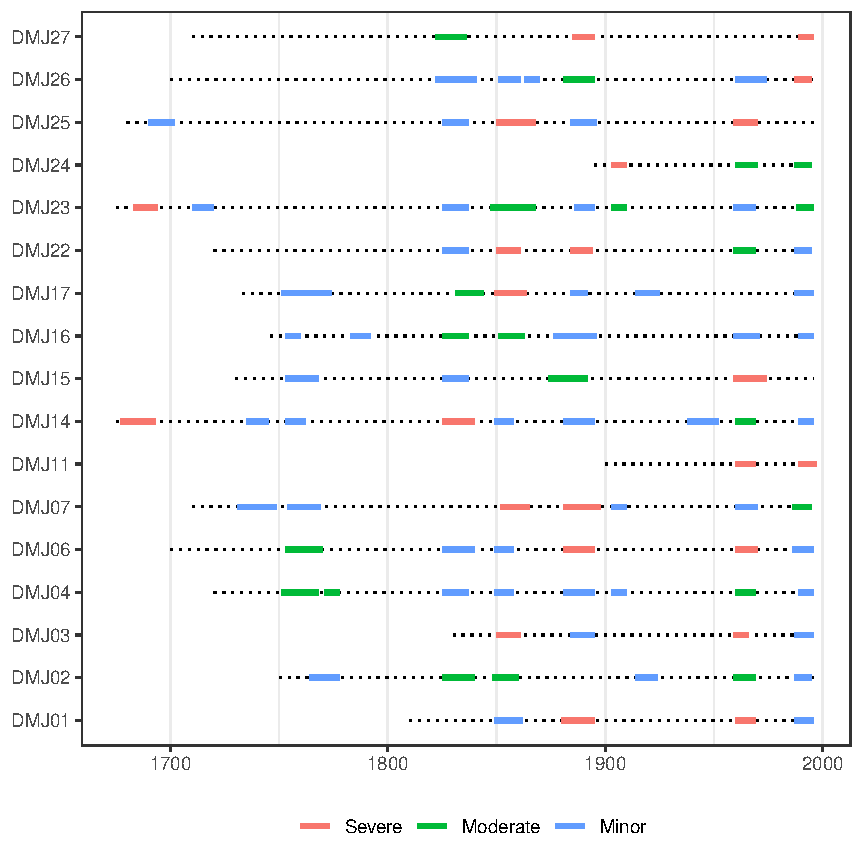
\includegraphics{../paper_elsevier/Output/tree-plot-default.pdf}
\caption{\label{fig:fig-defol}Default dfoliatR graphics for individual trees, produced by the `plot\_defol()' function. Dotted lines represent the series length for each tree and colored segments show periods of defoliation. Users can define the Cut-off values to determine severe-moderate-minor defoliation intensities, and use standard ggplot2 graphics parameters to adjust styles and themes.}
\end{figure}

\begin{figure}
\centering
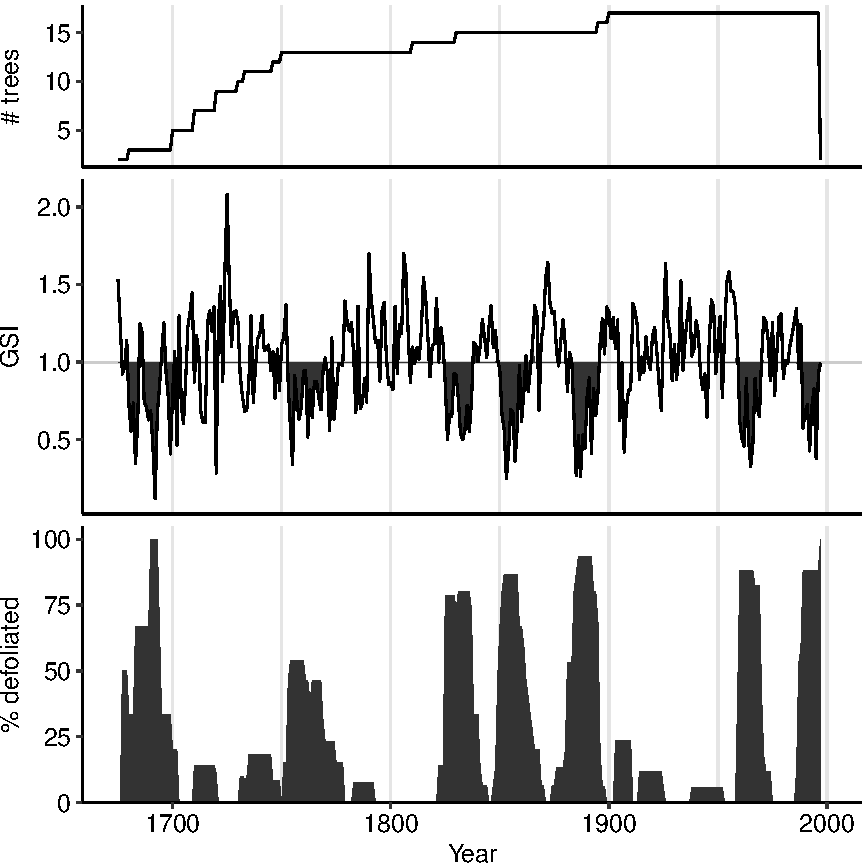
\includegraphics{../paper_elsevier/Output/site-plot.pdf}
\caption{\label{fig:fig-obr}Default graphic to show outbreak events at the DMJ site. Top panel shows the mean GSI through time, with inferred outbreak events filled. The middle panel shows the percent of trees defoliated, and the bottom panel shows the number of trees through time.}
\end{figure}

\begin{figure}
\centering
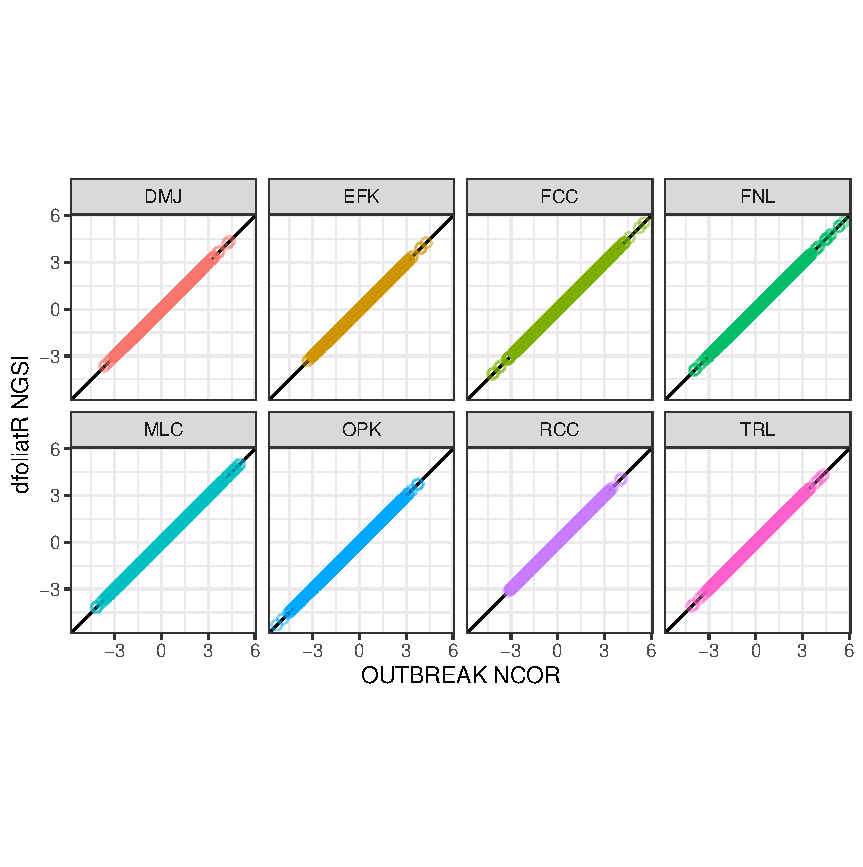
\includegraphics{../paper_elsevier/Output/plot-trees-df-obr.pdf}
\caption{\label{fig:df-obr-1-1}Comparison of disturbance indices between dfoliatR and OUTBREAK. Diagonal 1:1 lines show equal values.}
\end{figure}


\end{document}


